% Parent preamble: \usepackage{graphicx,amsmath,booktabs} (and \usepackage{caption} if customizing floats).
\section{Radial Schr\"odinger}

We first verify the accuracy of the spectral finite-element framework for the all-electron radial Schr\"odinger equation, which is obtained by setting $\hat{V}_{xc}=\widetilde{V}_H=0$ in the radial Kohn--Sham equation and admits analytical solutions. With a pure Coulomb nucleus $V_{\mathrm{nuc}}(r)=-Z/r$ and Hartree and exchange--correlation terms omitted, the radial eigenvalue problem is
\begin{equation}
    \label{eq:z92-radial-schrodinger}
    \left( -\frac{1}{2}\frac{\mathrm{d}^2}{\mathrm{d} r^2} -\frac{Z}{r} + \frac{l(l+1)}{2 r^2} \right) \widetilde{R}_{nl} = \lambda_{nl} \widetilde{R}_{nl} \,,
\end{equation}
with hydrogenic levels $\varepsilon_n=-Z^2/(2n^2)$~Ha. We consider $Z=92$ and compute all occupied eigenvalues using a domain size of $R_{\max}=40$~Bohr, an exponential mesh with shift $c=0$ and concentration parameter $a=100$, $N_{fe}=12$ finite elements, polynomial degree $p=20$, and quadrature order $q=60$. Figure~\ref{fig:z92-schrodinger-errors} shows the eigenvalue errors relative to the analytical values, demonstrating accuracies better than $10^{-10}$~Ha and confirming the accuracy of the spectral finite-element framework. The finite-element eigenvalues $\lambda_{nl}$ and their comparison to $\varepsilon_n$ are listed in Table~\ref{tab:z92-schrodinger-hydrogenic}.

\begin{figure}[!htbp]
    \centering
    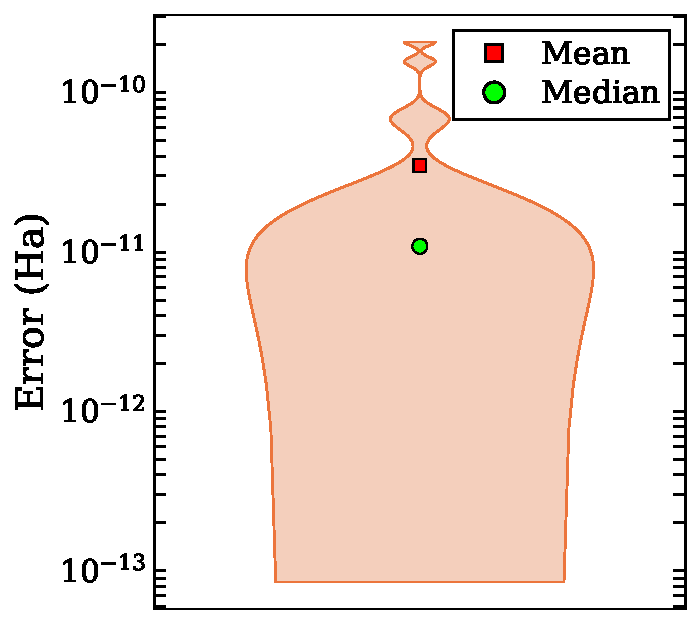
\includegraphics[width=0.48\textwidth]{../figures/test_z92_schrodinger_summary}
    \caption{Distribution of eigenvalue errors for the radial Schr\"odinger equation corresponding to $Z=92$.}
    \label{fig:z92-schrodinger-errors}
\end{figure}

\begin{table}[!htbp]
    \centering
    \footnotesize
    \setlength{\tabcolsep}{4pt}
    \caption{Occupied subshell eigenvalues for $Z=92$ (Ha); analytic $\varepsilon_n=-Z^2/(2n^2)$.}
    \label{tab:z92-schrodinger-hydrogenic}
    \begin{tabular}{@{}c c c r@{.}l r@{.}l r@{}}
        \toprule
        $n$ & $l$ & $g_{nl}$ & \multicolumn{2}{c}{numeric (Ha)} & \multicolumn{2}{c}{analytic (Ha)} & \multicolumn{1}{c}{Error (Ha)} \\
        \midrule
        1 & 0 & 2  & -4231 & 9999999998436 & -4232 & 0000000000000 & $1.56\times10^{-10}$ \\
        2 & 0 & 2  & -1057 & 9999999997924 & -1058 & 0000000000000 & $2.08\times10^{-10}$ \\
        2 & 1 & 6  & -1058 & 0000000000209 & -1058 & 0000000000000 & $2.09\times10^{-11}$ \\
        3 & 0 & 2  & -470  & 2222222222873 & -470  & 2222222222222 & $6.50\times10^{-11}$ \\
        3 & 1 & 6  & -470  & 2222222221507 & -470  & 2222222222222 & $7.15\times10^{-11}$ \\
        3 & 2 & 10 & -470  & 2222222222160 & -470  & 2222222222222 & $6.20\times10^{-12}$ \\
        4 & 0 & 2  & -264  & 5000000000234 & -264  & 5000000000000 & $2.34\times10^{-11}$ \\
        4 & 1 & 6  & -264  & 5000000000005 & -264  & 5000000000000 & $5.12\times10^{-13}$ \\
        4 & 2 & 10 & -264  & 5000000000092 & -264  & 5000000000000 & $9.15\times10^{-12}$ \\
        4 & 3 & 14 & -264  & 4999999999808 & -264  & 5000000000000 & $1.92\times10^{-11}$ \\
        5 & 0 & 2  & -169  & 2800000000126 & -169  & 2800000000000 & $1.26\times10^{-11}$ \\
        5 & 1 & 6  & -169  & 2799999999855 & -169  & 2800000000000 & $1.45\times10^{-11}$ \\
        5 & 2 & 10 & -169  & 2800000000001 & -169  & 2800000000000 & $8.53\times10^{-14}$ \\
        5 & 3 & 14 & -169  & 2799999999980 & -169  & 2800000000000 & $2.05\times10^{-12}$ \\
        6 & 0 & 2  & -117  & 5555555555597 & -117  & 5555555555556 & $4.11\times10^{-12}$ \\
        6 & 1 & 6  & -117  & 5555555555492 & -117  & 5555555555556 & $6.35\times10^{-12}$ \\
        6 & 2 & 10 & -117  & 5555555555598 & -117  & 5555555555556 & $4.21\times10^{-12}$ \\
        7 & 0 & 2  & -86   & 3673469387809 & -86   & 3673469387755 & $5.37\times10^{-12}$ \\
        \bottomrule
    \end{tabular}
\end{table}
